\chapter{Lorentztransformatie}
\vspace{-1cm}\begin{flushright}
{\it `Its not that I am smart, \\it's just that I stay with the problem longer'}\\ A. Einstein
\end{flushright}

Het tweede postulaat zoals geformuleerd in het voorgaande hoofdstuk is
duidelijk in tegenspraak met de Galileitransformatie en het is nu onze
taak een transformatie te vinden (het eerste postulaat zegt in feite
dat die er moet zijn) die in overeenstemming is met het tweede
postulaat.  Deze transformatie is in 1905 door Einstein gevonden en is
bekend geworden onder de naam Lorentztransformatie.  De afleiding
ervan is wiskundig gezien zeer eenvoudig, maar vereist, zoals we
zullen zien, nogal wat hersengymnastiek.

\section{Invariante interval}
We hebben gezien dat in de drie-dimensionale ruimte de co\"ordinaten van
twee punten $\vec{p}_1$ en $\vec{p}_2$ voor verschillende waarnemers,
waarvoor de onderlinge referentiesystemen zijn getransleerd, anders
zijn. Ze zijn het in deze drie-dimensionale ruimte wel eens over de
afstand tussen deze twee punten; dit is de invariant $\Delta r$.

We willen nu een dergelijke grootheid vinden voor een paar van `gebeurtenissen', een lengte in
de 3+1 dimensionele ruimte-tijd. Beschouw hiervoor persoon
$A$ die zich in de oorsprong van co\"{o}rdinaten-stelsel $S$ bevindt en
een persoon $B$ in de oorsprong van $S^{'}$.  $S^{'}$ beweegt
t.o.v. $S$ in de positieve $x$-richting met snelheid $v$.  Op $t=0$
valt de oorsprong van $S$ samen met die van $S^{'}$, d.w.z. vallen $A$
en $B$ samen.  Op $t=0$ ontsteekt $A$ heel eventjes een lampje
waardoor zich een bolvormige lichtgolf gaat uitbreiden.  $A$ bevindt
zich in het middelpunt van de bolvormige golf.  Een bol met straal $R$
en de oorsprong van het co\"{o}rdinatenstelsel als middelpunt wordt
beschreven door de formule :
\begin{displaymath}
x^{2} + y^{2} + z^{2} = R^{2}(t)
\end{displaymath}

% \begin{figure}[h]
% \begin{center}
% \mbox{\epsfxsize=8cm\epsffile{syllabus.pictures/spheres.eps}}
% \caption{Bolvormige lichtgolf}
% \label{f:lorentz1}
% \end{center}
% \end{figure}

\begin{figure}[ht]
\centering
%\includegraphics[width=1.00\textwidth]{syllabus.pictures/bolgolf}
\epsfig{file=bolgolf.pdf, width=\textwidth}
\caption{{\sl Bolvormige lichtgolf}}
\label{f:lorentz1}
\end{figure}


Voor een lichtgolf die zich uitbreidt met snelheid $c$ geldt na een tijd $t$: 
$R = ct$ en dus :
\begin{displaymath}
x^{2} + y^{2} + z^{2} = c^{2}t^{2}
\end{displaymath}
oftewel
\begin{equation}
\label{v:lorentz0a}
c^2 t^2 - x^{2} - y^{2} - z^{2} = 0
\end{equation}
Precies dezelfde redenering kunnen we echter volgen voor persoon $B$.
Ook $B$ denkt zich in het midden van de bolvormige lichtgolf te bevinden, het 
tweede postulaat zegt immers dat ook voor B het licht zich met snelheid $c$ 
uitbreidt.
Voor $B$, dus t.o.v. $S^{'}$, geldt nu geheel in analogie met hierboven :
\begin{displaymath}
x'^{2} + y'^{2} + z'^{2} = c^{2}t'^{2}
\end{displaymath}
oftewel
\begin{equation}
\label{v:lorentz0b}
c t'^2 - x'^{2} - y'^{2} - z'^{2} = 0
\end{equation}
In ons specifieke voorbeeld (beweging in de $x$-richting), geldt 
$(x \neq x^{'},$\newline $y = y^{'}, z = z^{'})$ dus moeten we wel concluderen 
$t \neq t^{'}$ (Aftrekken van \ref{v:lorentz0a} en \ref{v:lorentz0b} levert
$x^{2} - x'^{2} = c^{2}(t^{2} - t'^{2})$ en dus $t^{2} - t'^{2} \neq 0$) .
We komen al snel tot de conclusie dat de tijd voor $B$ anders 
verloopt dan voor $A$.\\
Bij elk referentiestelsel hoort niet alleen een eigen plaatsmeting maar 
ook een eigen tijdmeting.
Hoe plaats en tijd van een bepaald natuurkundig verschijnsel zoals geldend 
in $S$ worden uitgedrukt in plaats en tijd van hetzelfde verschijnsel 
t.o.v. $S^{'}$ wordt gegeven door de Lorentztransformatie.

In elk geval weten we al (zie boven) dat zal moeten gelden:
\begin{equation}
\label{v:lorentz1}
c^2 t'^2 - x'^{^{2}} - y'^{^{2}} - z'^{^{2}} = c^2 t^2 - x^{2} - y^{2} - z^{2} 
\end{equation}
We zeggen dat de grootheid $c^2 t^2 - x^{2} - y^{2} - z^{2}$
{\sl invariant} is onder Lorentztransformaties. 

Iets algemener kunnen we twee gebeurtenissen A en B in het stelsel $S$ beschouwen, met onderling tijdsverschil $\Delta t$ en
ruimteverschillen $(\Delta x,\Delta y, \Delta z)$. We hebben laten zien dat de afstand tussen deze twee gebeurtenissen,
gedefinieerd als 
\begin{eqnarray}
(\Delta s)^2 & \equiv & (c \Delta t)^2 - (\Delta r)^2 \\
             & \equiv & (c \Delta t)^2 - (\Delta x)^2 - (\Delta y)^2 - (\Delta z)^2
\end{eqnarray}
{\it invariant} is onder het relativiteitsprincipe van Einstein.
Dit invariante interval staat centraal in de speciale relativiteitstheorie.

\subsection{Nogmaals de lichtklok}
In paragraaf~\ref{s:lichtklok} hebben we de lichtklok
ge\"introduceerd. In het referentiesysteem van D waarin de klok stil staat, tikte de klok met
tikken van $(c\Delta t)=1$ m (elke 3.3 ns), en de afgelegde afstand in de $x$-richting tussen twee tikken is $\Delta
x=0$. Het invariante interval tussen twee tikken wordt daarmee $(\Delta
s)^2 = (c \Delta t)^2-(\Delta x)^2 = 1 $m$^2$. 

In het referentiestelsel
van E is $c \Delta t' = \gamma$(1 m) en de afgelegde afstand afstand in $x$ tussen twee tikken wordt
gegeven door de snelheid $v$ te vermenigvuldigen met de het tijdsverschil $\Delta t'$, $\Delta x' = \gamma v$(1 m)$/c$. Het
interval in E's referentiesysteem wordt hiermee $(\Delta s')^2
=\gamma^2(1-v^2/c^2)$(1 m$^2$). Omdat geldt dat $\gamma\equiv
1/\sqrt{(1-v^2/c^2)}$, wordt het interval hiermee $(\Delta s')^2 =
(\Delta s)^2 = 1$ m$^2$. We hebben laten zien dat het interval
dezelfde waarde heeft voor waarnemer D en waarnemer E. Voor elke
andere waarnemer die in een referentiesysteem zit, geldt dat hij
andere tijdverschillen meet, en andere ruimte afstanden vindt. Maar het
interval $(\Delta s)^2$ blijft altijd 1 m$^2$.

\section{De eigentijd en eigenlengte}
De {\sl eigentijd} $\Delta \tau$ tussen twee gebeurtenissen is het
tijdsinterval zoals waargenomen in een co\"ordinatenstelsel waarin de
twee gebeurtenissen op dezelfde positie plaatsvinden. Dit is niet in
alle gevallen mogelijk.  Zoals in bovenstaand voorbeeld duidelijk is
gemaakt, is het invariante interval tussen twee gebeurtenissen $c$
maal de eigentijd, of $c\Delta \tau = \sqrt{(\Delta s)^2}$. De
eigentijd is het tijdsinterval in het co\"ordinatenstelsel van D, het
stelsel waarin de lichtklok stil staat. De eigentijd is de tijd zoals
die verloopt voor de waarnemer zelf; het is zijn {\it eigen} tijd.


 Als het interval positief is, is er altijd een co\"ordinatenstelsel te
vinden waarin de positie van de gebeurtenissen hetzelfde is. Dit omdat
een positief interval betekent $|c \Delta t | > | \Delta r|$, dus een
referentiesysteem dat beweegt met een snelheid $\vec{v}=(\Delta
\vec{r})/(\Delta t)$ transformeert  de gebeurtenissen naar hetzelfde punt. En 
de  snelheid is kleiner dan die van het licht. 

Als het interval tussen twee gebeurtenissen kleiner is dan nul, d.w.z.
$(\Delta s)^2 < 0$, is het nog steeds een invariant. Maar er kan in dit
geval geen co\"ordinatenstelsel gevonden worden waarin beide
gebeurtenissen op dezelfde positie plaatsvinden. Dit
co\"ordinatenstelsel is er niet - het zou sneller dan met de lichtsnelheid
moeten bewegen ten opzichte van het stelsel van de twee
gebeurtenissen. Soms wordt hiervoor de {\it eigenlengte} ge\"introduceerd, $\Delta \lambda$, als
de ruimtelijke afstand tussen twee gebeurtenissen in een referentiesysteem waarin de gebeurtenissen
gelijktijdig plaatsvinden. Dit kan alleen als het interval negatief is, en de eigenlengte wordt
dan $\Delta \lambda = \sqrt{|(\Delta s)^2|}$. 

Het interval $(\Delta s)^2$ kan natuurlijk ook precies gelijk zijn
aan nul. Dit is het geval wanneer $(c \Delta t)^2 = (\Delta r)^2$,
met andere woorden, wanneer de wereldlijn overeenkomt met die van het
licht. Omdat de lichtsnelheid in elk co\"ordinatenstelsel dezelfde is,
is dit interval weer gelijk aan nul in elk co\"ordinatenstelsel.

Intervallen $(\Delta s)^2=0$ noemen we {\sl `lichtachtig'}. Intervallen $(\Delta s)^2>0$ noemen we {\sl `tijdachtig'} en
intervallen $(\Delta s)^2< 0$ noemen we {\sl `ruimteachtig'}. Deze intervallen hebben verschillende eigenschappen
met betrekking tot causaliteit; we komen hier op terug.



\section{De Lorentztransformatie, een eenvoudige afleiding}
We defini\"{e}ren co\"{o}rdinatenstelsels $S$ en $S^{'}$ weer als voorheen:
$S^{'}$ beweegt t.o.v. $S$ met constante snelheid $v$ in de positieve 
$x$-richting.
Op $t = t^{'} = 0$ valt de oorsprong van $S$ samen met die van $S^{'}$.
Een lichtflits, uitgezonden in de positieve $x$-richting, bevindt zich op 
plaats $x = ct$, d.w.z. $x - ct = 0$.
T.o.v. $S^{'}$ geldt $x' - ct^{'} = 0$ (zelfde $c$, tweede postulaat!).
Aan beide vergelijkingen wordt voldaan als geldt:
\begin{equation}
x^{'} - ct^{'} = \lambda (x - ct)
\end{equation}
waar $\lambda$ een constante is die we nog moeten bepalen.
We kunnen uiteraard dezelfde redenering volgen voor een lichtflits die wordt 
uitgezonden in de negatieve $x$-richting.
Dan vinden we dat moet gelden:
\begin{equation}
\label{v:lorentz2}
x^{'} + ct^{'} = \mu (x + ct)
\end{equation}
Ook $\mu$ is een nog nader te bepalen constante.
Optellen resp. aftrekken van \ref{v:lorentz1} en \ref{v:lorentz2} levert:
\begin{displaymath}
ct^{'} = \frac{\lambda + \mu}{2} ct - \frac{\lambda - \mu}{2} x \\
\end{displaymath}
\begin{displaymath}
x^{'} = \frac{\lambda + \mu}{2} x - \frac{\lambda - \mu}{2} ct 
\end{displaymath}
We defini\"{e}ren twee nieuwe constanten, $a = \frac{\lambda + \mu}{2}$
en $b = \frac{\lambda - \mu}{2}$ en verkrijgen de overzichtelijke 
vergelijkingen:
\begin{equation}
\label{v:lorentz4}
ct^{'} = act - bx
\end{equation}
\begin{equation}
\label{v:lorentz3}
x^{'} = ax - bct
\end{equation}
waar we nog steeds als taak hebben om $a$ en $b$ te bepalen (d.w.z. uit te 
drukken in $v$, de parameter die de transformatie defini\"{e}ert.)

Voor de oorsprong van $S^{'}$ geldt t.o.v. $S$:
\begin{displaymath}
x = vt
\end{displaymath}
en t.o.v. $S^{'}$ uiteraard:
\begin{displaymath}
x^{'} = 0
\end{displaymath}
Invullen in \ref{v:lorentz3} levert dan dat moet gelden:
\begin{equation}
\label{v:lorentz5}
v = \frac{b}{a}c
\end{equation}

% \begin{figure}
% \begin{center}
% \mbox{\epsfxsize=8cm\epsffile{syllabus.pictures/ruler.eps}}
% \caption{Meetlat}
% \label{f:lorentz2}
% \end{center}
% \end{figure}

\begin{figure}[ht]
\centering
\epsfig{file=ruler.pdf, width=0.5\textwidth}
%\includegraphics[width=.5\textwidth]{syllabus.pictures/ruler}
\caption{Meetlat}
\label{f:lorentz2}
\end{figure}


Nu gebruiken we het relativiteitsprincipe in de volgende redenering: 
een meetlat die langs de $x^{'}$-as ligt, in rust t.o.v. $S^{'}$, 
heeft, gezien vanuit $S$ dezelfde lengte als diezelfde meetlat, gelegen 
langs de $x$-as, in rust t.o.v. $S$, gezien vanuit $S^{'}$!
\begin{itemize}
\item \underline{Observatie 1} \\
Op een zekere tijd $t$ in $S$ kunnen we dus de lengte van de meetlat 
t.o.v. $S^{'}$ bepalen, bijvoorbeeld op \underline{$t = 0$}.
We vinden dan met behulp van \ref{v:lorentz3}:
\begin{displaymath}
x^{'} = ax
\end{displaymath}
\item \underline{Observatie 2} \\
Omgekeerd vinden we op \underline{$t^{'} = 0$}, m.b.v. \ref{v:lorentz3} en 
\ref{v:lorentz4} en gebruikmakend van \ref{v:lorentz5}:
\begin{displaymath}
x^{'} = a(1 - \frac{v^{2}}{c^{2}})x
\end{displaymath}
\end{itemize}
Wanneer we zeggen dat de lengte van de meetlat $l_0$ is, dan bedoelen we: 
de lengte is $l_{0}$ in het systeem waarin de meetlat in rust is.
Observatie 1 (meetlat in rust in  $S^{'}$ gefotografeerd vanuit $S$) leert dan:
\begin{displaymath}
l_{0} = al
\end{displaymath}
waar $l$ dus de lengte t.o.v. $S$ is, d.w.z. ten opzichte van het 
co\"{o}rdinatenstelsel waarin de lat beweegt.
Observatie 2 ($S$ gefotografeerd vanuit $S^{'}$) levert op:
\begin{displaymath}
l = a(1-\frac{v^{2}}{c^{2}})l_{0}
\end{displaymath}
Het combineren van deze resultaten levert dan het volgende resultaat op:
\begin{displaymath}
a = \frac{1}{\sqrt{1-\frac{v^{2}}{c^{2}}}}
\end{displaymath}
Degenen die achterdochtig worden van deze nogal veel woorden kostende 
afleiding vinden de volgende beschouwing misschien eleganter.\\
We pikken de afleiding op na formule \ref{v:lorentz5} en schrijven 
\ref{v:lorentz3} en \ref{v:lorentz4} als :
\begin{equation}
\label{v:lorentz7}
ct^{'} = a(ct - \frac{v}{c}x)
\end{equation}
\begin{equation}
\label{v:lorentz6}
x^{'} = a(x - vt)
\end{equation}
Bovenstaande transformatie geldt als $S^{'}$ beweegt in de positieve 
$x$-richting, dus met snelheid $+v$, t.o.v. $S$.
Maar we kunnen ook $S^{'}$ als rustsysteem kiezen en $S$ als het bewegende 
systeem zien dat t.o.v. $S^{'}$ naar links beweegt, d.w.z. met snelheid $-v$.
De {\sl inverse} transformatie wordt dan onmiddellijk uit de bovenstaande 
verkregen door `accenten te verwisselen' (de accenten slaan immers op het 
bewegende systeem en die rol wordt nu 
overgenomen door $S$) en door $v$ te vervangen door $-v$. 
Dit levert:
\begin{equation}
ct = a(ct^{'} + \frac{v}{c}x^{'})
\label{v:lorentz9}
\end{equation}
\begin{equation}
\label{v:lorentz8}
x = a(x^{'} + vt^{'})
\end{equation}
(Merk op dat deze redenering alleen correct is als $a$ ongevoelig is voor 
het teken van $v$. 
Gelukkig blijkt dat zo te zijn volgens het eerste postulaat.)
Indien we \ref{v:lorentz8} en \ref{v:lorentz9} gebruiken om $t^{'}$ in $t$ 
en $x$ uit te drukken en het resultaat vervolgens vergelijken met 
\ref{v:lorentz7} vinden we 
\begin{displaymath}
a = \frac{1}{\sqrt{1 - \frac{v^{2}}{c^{2}}}}
\end{displaymath}
Aldus hebben we de Lorentztransformatie gevonden:
\begin{displaymath}
ct^{'} = \frac{ct - x \frac{v}{c}}{\sqrt{1 - \frac{v^{2}}{c^{2}}}}
\end{displaymath}
\begin{displaymath}
x^{'} = \frac{x - vt}{\sqrt{1 - \frac{v^{2}}{c^{2}}}}
\end{displaymath}
In ons specifieke geval, relatieve beweging langs de $x$-as, geldt verder
\begin{displaymath}
y^{'} = y
\end{displaymath}
\begin{displaymath}
z^{'} = z
\end{displaymath}
Ga nu na dat formule \ref{v:lorentz1} inderdaad klopt, dat wil zeggen, dat het inderdaad het `invariante interval' $(\Delta s)^2$ invariant laat! Samenvattend:
\begin{quote}
Lorentztransformaties verbinden, net als Galileitransformaties,
inertiaalsystemen op een manier die in overeenstemming is met het
relativiteitsprincipe en het lichtpostulaat. In tegenstelling tot
Galileitransformaties laten ze de lichtsnelheid invariant. Hiermee
zijn ze in overeenstemming met de Maxwell-theorie van het
elektromagnetisme.
\end{quote}

\subsection{Notatie}
We hadden al ingevoerd dat 
\begin{eqnarray}
\beta & = & \frac{v}{c} \\
\gamma & = & \frac{1}{\sqrt{1-\beta^2}}
\end{eqnarray}
De Lorentztransformatie langs de $x$-as wordt hiermee geschreven als:
\begin{eqnarray}
\label{v:lorentz11}
ct' &  = & \gamma (ct - \beta x) \\ \label{v:lorentz10}
x'  &  = & \gamma (x -  \beta ct)\\
y'  & = & y \\
z' & = & z 
\end{eqnarray}
oftewel in matrix vorm\footnote{Voor een overzicht van matrix algebra wordt u doorverwezen naar
de cursus lineare algebra. Kortweg geldt dat een kolom-vector vermenigvuldigd met een matrix een nieuwe kolom-vector oplevert volgens de regel
\[
\left( \begin{array}{c} y_0 \\ y_1 \\ y_2 \\ y_3 \end{array} \right) =
\left( \begin{array}{cccc} a_{00} & a_{01} & a_{02} & a_{03} \\ 
                           a_{10} & a_{11} & a_{12} & a_{13} \\ 
                           a_{20} & a_{21} & a_{22} & a_{23} \\ 
                           a_{30} & a_{31} & a_{32} & a_{33} \end{array} \right) 
\left( \begin{array}{c} x_0 \\ x_1 \\ x_2 \\ x_3 \end{array} \right) =
\left( \begin{array}{c} a_{00} x_0 + a_{01} x_1 + a_{02} x_2 + a_{03} x_3 \\ 
                        a_{10} x_0 + a_{11} x_1 + a_{12} x_2 + a_{13} x_3 \\ 
                        a_{20} x_0 + a_{21} x_1 + a_{22} x_2 + a_{23} x_3 \\ 
                        a_{30} x_0 + a_{31} x_1 + a_{32} x_2 + a_{33} x_3  \end{array} \right). 
\]}.
\begin{equation}
\left( \begin{array}{c} ct' \\ x' \\ y' \\ z' \end{array} \right) =
\left( \begin{array}{cccc} \gamma & -\gamma \beta & 0 & 0  \\ -\gamma\beta & \gamma & 0 & 0  \\ 0 & 0 & 1 & 0  \\ 0 & 0 & 0 & 1 
\end{array} \right) 
\left( \begin{array}{c} ct \\ x \\ y \\ z \end{array} \right) 
\end{equation}
De inverse Lorentztransformatie wordt dan 
\begin{equation}\label{v:lorentz12}
\left( \begin{array}{c} ct \\ x \\ y \\ z \end{array} \right) =
\left( \begin{array}{cccc} \gamma & \gamma \beta & 0 & 0  \\ \gamma\beta & \gamma & 0 & 0  \\ 0 & 0 & 1 & 0  \\ 0 & 0 & 0 & 1 
\end{array} \right) 
\left( \begin{array}{c} ct' \\ x' \\ y' \\ z' \end{array} \right) 
\end{equation}
De ruimte-tijd symmetrie, d.w.z. de verwevenheid van $x$ en $ct$, de 
volstrekt gelijkwaardige rol van beide grootheden, is in deze notatie heel 
duidelijk.

\section{Lorentztransformaties}
De Lorentztransformaties (LT) zijn belangrijk en verdienen een
discussie. De LT transformeren de afstanden $(c\Delta t, \Delta x,
\Delta y, \Delta z)$ tussen de co\"ordinaten van twee gebeurtenissen in
een co\"ordinatenstelsel naar de afstanden $(c\Delta t', \Delta x',$ $
\Delta y', \Delta z')$ in een ander co\"ordinatenstelsel. Het betekent
dat als de LT direct op de co\"ordinaten van \'e\'en gebeurtenis
toegepast worden, impliciet de andere gebeurtenis op co\"ordinaten
$(0,0,0,0)$ in beide stelsels wordt genomen. De transformaties waarbij
de snelheid van een co\"ordinatensysteem anders wordt, noemen we een
{\it boost}. Deze boost-transformaties vormen het hart van de speciale
relativiteitstheorie.

We kunnen eenvoudig de consistentie van de LT laten zien door eerst een
co\"ordinatensysteem te transformeren met snelheid $v$, en vervolgens
weer terug te transformeren met snelheid $-v$. We zullen uiteindelijk
datgene weer terug moeten vinden met waarmee we begonnen waren. Met
andere woorden: LT's met gelijke maar tegengestelde
snelheden moeten elkaars {\sl inverse} zijn. Als we van richting
veranderen, d.w.z. $v\rightarrow -v$, dan wordt $\beta \rightarrow
-\beta$ en $\gamma \rightarrow \gamma$. De transformatie van de
co\"ordinaten $(ct,x)$ naar $(ct',x')$ en weer terug naar co\"ordinaten
$(ct'',x'')$ wordt dan
\begin{eqnarray} 
ct'' & = & \gamma ct' + \beta \gamma x' \\ \nonumber
     & = & \gamma ( \gamma ct -\beta \gamma x) + \beta \gamma (-\beta \gamma ct + \gamma x) \\ \nonumber
     & = & \gamma^2 (ct-\beta x - \beta^2 ct + \beta x)\\ \nonumber
     & = & \gamma^2 (1-\beta^2) ct \\ \nonumber
     & = & ct \\
x'' & = & \beta \gamma ct' + \gamma x' \\ \nonumber
     & = & \beta \gamma ( \gamma ct -\beta \gamma x) + \gamma (-\beta \gamma ct + \gamma x) \\\nonumber
     & = & \gamma^2 (\beta ct-\beta^2 x - \beta ct + x)\\\nonumber
     & = & \gamma^2 (1-\beta^2) x \\\nonumber
     & = & x 
\end{eqnarray}
dus is inderdaad de transformatie langs snelheid $-v$ de inverse van de transformatie langs $v$.

De groep van alle LT's bevat alle lineare transformaties die het interval $(\Delta s)^2$ 
invariant laat. Dit betekent dat ook rotaties in de ruimte, zonder `boost', bij de LT's horen. De
rotatie om de $z$-as met hoek $\theta$ is een voorbeeld:
\begin{equation}
\left( \begin{array}{cccc} 
    1 & 0 & 0 & 0 \\
    0 & \cos\theta & -\sin\theta & 0 \\
    1 & -\sin\theta & \cos\theta & 0 \\
    0 & 0 & 0 & 1 \end{array} \right)
\end{equation}

De LT's bevatten ook de `boost' translaties tussen twee co\"ordinatenstelsels $S$ en $S'$ langs
 willekeurige richting $\vec{v}=(v_x,v_y,v_z)$. 
Zonder verdere afleiding geven we het resultaat
\begin{equation}
\left( \begin{array}{cccc} 
    \gamma & -\gamma\beta_x & -\gamma\beta_y & -\gamma\beta_z \\
    -\gamma\beta_x & 1+\frac{(\gamma-1)\beta_x^2}{\beta^2} & 1+\frac{(\gamma-1)\beta_x\beta_y}{\beta^2} & 1+\frac{(\gamma-1)\beta_x\beta_z}{\beta^2} \\
    -\gamma\beta_y & 1+\frac{(\gamma-1)\beta_x\beta_y}{\beta^2} & 1+\frac{(\gamma-1)\beta_y^2}{\beta^2} & 1+\frac{(\gamma-1)\beta_y\beta_z}{\beta^2}\\
    -\gamma\beta_z & 1+\frac{(\gamma-1)\beta_x\beta_z}{\beta^2} & 1+\frac{(\gamma-1)\beta_y\beta_z}{\beta^2} & 1+\frac{(\gamma-1)\beta_z^2}{\beta^2}
 \end{array} \right)
\end{equation}
waarbij
\begin{eqnarray}
\beta_x & = & v_x/c \\ \nonumber
\beta_y & = & v_y/c \\ \nonumber
\beta_z & = & v_z/c \\ \nonumber
\beta^2 & = & \beta_x^2 + \beta_y^2 + \beta_z^2 \\\nonumber
\gamma & = & (1-\beta_x^2-\beta_y^2-\beta_z^2)^{-1/2}.\nonumber
\end{eqnarray}
Samenstellingen van verschillende LT's zijn zelf ook weer LT's.



\section{Lorentzcontractie}
In paragraaf~\ref{s:contractie} hebben we laten zien dat bewegende
stokken korter worden. We zullen dit nu nogmaals laten zien, maar nu
maken we gebruik van de Lorentztransformatie voor de afleiding van het
resultaat. 

Daartoe bekijken we een bewegende stok. De stok
heeft t.o.v. het co\"{o}rdinatenstelsel waarin hij in rust is een
lengte $l_{0}$.  Wat is dan de lengte t.o.v. het
co\"{o}rdinatenstel-sel waarin hij beweegt?  Wij nemen een stok die
langs de $x^{'}$-as ligt, met het linker uiteinde in de oorsprong van
$S^{'}$ en die in rust is t.o.v. $S^{'}$.  Voor de
$x^{'}$-co\"{o}rdinaat van het rechter uiteinde geldt dus:
\begin{displaymath}
x^{'}_{R} = l_{0}
\end{displaymath}
en voor het linker uiteinde geldt:
\begin{displaymath}
x^{'}_{L} = 0
\end{displaymath}
De overeenkomstige $x$-co\"{o}rdinaten in $S$ volgen uit \ref{v:lorentz12}:
\begin{displaymath}
x_{R} = \gamma (l_{0} + \beta ct^{'}_{R})
\end{displaymath}
\begin{displaymath}
x_{L} = \gamma \beta ct^{'}_{L}
\end{displaymath}
De lengte $l$ t.o.v. $S$ is:
\begin{displaymath}
l = x_{R} - x_{L}
\end{displaymath}
\begin{equation}
\label{v:vier2}
l = \gamma \{l_{0} + \beta c(t^{'}_{R} - t^{'}_{L})\}
\end{equation}
Het is heel belangrijk dat we ons realiseren dat de lengte $l$ t.o.v. $S$ 
gelijk is aan $x_{R} - x_{L}$, waar $x_{R}$ en $x_{L}$ op 
{\sl dezelfde tijd t.o.v. $S$} bepaald worden, 
dus $t_{R} = t_{L}$.
Met behulp van \ref{v:lorentz11} volgt dan:
\begin{displaymath}
ct^{'}_{R} = \gamma (ct_{R} - \beta x_{R})
\end{displaymath}
\begin{displaymath}
ct^{'}_{L} = \gamma (ct_{L} - \beta x_{L}) 
\end{displaymath}
Aftrekken van de vergelijkingen levert:
\begin{displaymath}
c(t^{'}_{R} - t^{'}_{L}) = -\gamma \beta (x_{R} - x_{L}) = -\gamma \beta l
\end{displaymath}
Dit resultaat vullen we in in \ref{v:vier2} en we vinden:
\begin{displaymath}
l = \gamma (l_{0} - \gamma \beta ^{2} l)
\end{displaymath}
\begin{displaymath}
l (1 + \beta ^{2} \gamma ^{2}) = \gamma l_{0}
\end{displaymath}
Aangezien $\gamma ^{2} = \frac{1}{1 - \beta ^{2}}$ (definitie) volgt nu:
\begin{equation}
\label{v:vier3}
l = \frac{l_{0}}{\gamma}
\end{equation}
$l$ is dus kleiner dan $l_{0}$: de bewegende stok is korter, precies
zoals we al eerder gevonden hadden. Dit effect gaat onder de naam {\sl
Lorentzcontractie}.

\section{Optellen van snelheden}
We kunnen nu de juiste formule afleiden voor het optellen van
snelheden, zoals we in de inleiding al bespraken.  Als A met een
snelheid $+u$ in de $x$-richting beweegt ten opzichte van B, en A
gooit een appel met snelheid $+v$ in de $x$-richting ten opzichte van
zichzelf, met welke snelheid ziet dan waarnemer B de appel voorbij
vliegen?  We hadden al gezien dat het klassieke antwoord $w=u+v$
onjuist is. Het juiste antwoord kan worden afgeleid met behulp van de
Lorentztransformaties. Noem hiervoor het moment waarop A de appel gooit $T$, en neem dit als de
 oorsprong van beide co\"ordinatenstelsels, zodat $(ct_T,x_T)=(ct'_T,x'_T)=(0,0)$, waarbij
het stelsel van A aangegeven wordt met accenten. Stel nu verder voor dat een tijdje $t'$ later in het co\"ordinatenstelsel
van A de appel explodeert. De co\"ordinaten van de explosie worden hiermee $(ct',vt')$ in het stelsel van A.
In het co\"ordinatenstelsel in rust ten opzichte van B vind gebeurtenis $T$ ook plaats in de oorsprong, en de
explosie van de appel vind plaats met co\"ordinaten verkregen uit de Lorentztransformatie:
\begin{eqnarray}
ct & = & \gamma c t' + \beta \gamma vt' \\ \nonumber
x & = & \beta \gamma c t' + \gamma vt'
\end{eqnarray}
De snelheid $w$ zoals B die meet is eenvoudigweg $x/t$ oftewel
\begin{eqnarray}
w &=& c\frac{\beta\gamma c t'+\gamma v t'}{\gamma c t'+\beta \gamma vt'} \\\nonumber
 &=& \frac{u+v}{1+uv/c^2}
\end{eqnarray}
en is dus kleiner dan $u+v$.


We gaan nu hetzelfde resultaat opnieuw afleiden, maar dan iets
formeler. We zullen daarbij vinden dat bij een translatie langs de
$x$-as niet alleen de formule voor het optellen van snelheid in de
$x$-richting, maar ook in de $y$- en $z$-richting moet worden
aangepast.

Per definitie geldt voor de snelheid:
\begin{displaymath}
V'_{x} = \frac{dx'}{dt'}
\end{displaymath}
Vul nu in (formule \ref{v:lorentz10}):
\begin{displaymath}
x' = \gamma (x - \beta ct)
\end{displaymath}
dan vinden we:
\begin{displaymath}
V'_{x} = \gamma \frac{dx}{dt'} - \beta \gamma c \frac{dt}{dt'}
\end{displaymath}
Verder geldt (`kettingregel'):
\begin{displaymath}
\frac{dx}{dt'} = \frac{dx}{dt} \frac{dt}{dt'}
\end{displaymath}
en dus vinden we:
\begin{displaymath}
V'_{x} = (\gamma \frac{dx}{dt} - \beta \gamma c)\frac{dt}{dt'}
\end{displaymath}
en aangezien
\begin{displaymath}
V_{x} = \frac{dx}{dt}
\end{displaymath}
wordt dit
\begin{equation}
\label{v:optel1}
V'_{x} = (\gamma V_{x} - \beta \gamma c)\frac{dt}{dt'}
\end{equation}
Nu gebruiken we (formule \ref{v:lorentz12}):
\begin{displaymath}
ct = \gamma (ct' + \beta x')
\end{displaymath}
waaruit volgt:
\begin{displaymath}
\frac{dt}{dt'}  = \gamma + \frac{\beta \gamma}{c} V'_{x}
\end{displaymath}
invullen hiervan in formule \ref{v:optel1} levert dan:
\begin{displaymath}
V'_{x} = \frac{V_{x} - \beta c}{1 - \frac{\beta}{c} V_{x}}
\end{displaymath}
Merk op, dat als $V_{x} = c$ we vinden dat ook $V'_{x} = c$.
We kunnen een lichtstraal dus niet inhalen, geheel en al in overeenstemming
met het eerste postulaat\\
Ook $V'_{y}$ en $V'_{z}$ blijken (anders dan $y'$ en $z'$) onder een 
Lorentztransformatie in de $x$-richting te veranderen:
\begin{eqnarray*}
V'_{y} & = &  \frac{dy'}{dt'} = \frac{dy}{dt'} = \frac{dy}{dt} \frac{dt}{dt'} \\
       & = &  V_{y} (\gamma + \frac{\beta \gamma}{c} V'_{x})
\end{eqnarray*}
Hieruit vinden we m.b.v. de transformatieformule voor $V'_{x}$ hierboven:
\begin{equation}\label{e:vy}
V'_{y} = \frac{V_{y}}{\gamma (1 - \frac{\beta}{c} V_{x})}
\end{equation}
en net zo:
\begin{equation}
V'_{z} = \frac{V_{z}}{\gamma (1 - \frac{\beta}{c} V_{x})}
\end{equation}


 
\section{Intermezzo: Alternatieve Lorentztransformatie}
In deze paragraaf willen we nogmaals laten zien dat een willekeurig voorwerp nooit sneller dan $c$ kan bewegen. Hiertoe gaan we eerst de Lorentztransformaties op een andere manier parameterizeren. Deze paragraaf kan overgeslagen worden en dient hier slechts `ter lering ende vermaak'.

Bekijk verschillende  Lorentztransformaties langs de $x$-richting.
Beschouw drie inertiaalsystemen $S$, $S'$ en $S''$, met standaard
Lorentztransformaties $S\rightarrow S'$ en $S'\rightarrow S''$ met
onderlinge snelheden $\beta_1$ en $\beta_2$ respectievelijk. We
noteren de snelheid tussen stelsel $S\rightarrow S''$ met $\beta$, dus
zonder index. We hebben eerder gevonden dat de optelformule voor
snelheden geeft:
\begin{equation}\label{e:b1}
\beta = \frac{\beta_1  + \beta_2 }{1+\beta_1 \beta_2}  
\end{equation}

De snelheden $\beta_1$ en $\beta_2$ tellen dus niet zomaar op tot
$\beta$. Het is daarom handig om een andere parameters voor de
snelheid in te voeren, die wel opgeteld kan worden.  We
defini\"eren nu een nieuwe grootheid $\phi$ als volgt:
\begin{equation}\label{e:b2}
\phi = \frac{1}{2}\ln\left(\frac{1+\beta}{1-\beta}\right)
\end{equation}
We hebben dus voor de transformatie $S\rightarrow S'$ de parameter $\phi_1$ als
\[
\phi_1 = \frac{1}{2}\ln\left(\frac{1+\beta_1}{1-\beta_1}\right)
\]
en voor $S'\rightarrow S''$
\[
\phi_2 = \frac{1}{2}\ln\left(\frac{1+\beta_2}{1-\beta_2}\right)
\]

Nu vullen we in vergelijking~\ref{e:b2} de uitdrukking~\ref{e:b1} in:
\begin{equation}
\phi = \frac{1}{2}\ln\left( \frac{1+ \frac{\beta_1 + \beta_2}{1+\beta_1 \beta_2}}{1-\frac{\beta_1 + \beta_2}{1+\beta_1 \beta_2}  }\right)  
\end{equation}
en vereenvoudigen dit tot
\begin{equation}
\phi = \frac{1}{2}\ln\left( \frac{1+ \beta_1 \beta_2 + (\beta_1 + \beta_2)}{1 + \beta_1 \beta_2 -(\beta_1 + \beta_2)}  \right) = \frac{1}{2}\ln\left(\left(\frac{1+\beta_1}{1-\beta_1}\right)  \left(\frac{1+\beta_2}{1-\beta_2}\right)\right) = \phi_1 + \phi_2  
\end{equation}
We hebben dus gevonden dat de parameter $\phi$ bij opeenvolgende Lorentztransformaties in dezelfde richting optellen. We noemen dit {\it additief}; de parameter $\phi$ is additief. 

We kunnen hiermee de Lorentztransformaties in termen van $\phi$ schrijven. Uit de definitie van $\phi$ volgt:
\begin{equation}
e^{\phi} = \sqrt{\left(\frac{1+\beta}{1-\beta}\right)}=\sqrt{\frac{(1+\beta)^2}{1-\beta^2}}=\sqrt{\gamma^2(1+\beta)^2}=\gamma(1+\beta)
\end{equation} 
en evenzo
\begin{equation}
e^{-\phi} = \sqrt{\left(\frac{1-\beta}{1+\beta}\right)}=\gamma(1-\beta)
\end{equation} 
De hyperbolische trigonometrische functies zijn gedefini\"eerd als
\begin{eqnarray}
\sinh \alpha & = & \frac{1}{2}\left( e^{\alpha}-e^{-\alpha}\right) \\
\cosh \alpha & = & \frac{1}{2}\left( e^{\alpha}+e^{-\alpha}\right) \\
\tanh \alpha & = & \frac{\sinh\alpha}{\cosh\alpha} = 
\left(e^{\alpha}-e^{-\alpha}\right)/ \left(e^{\alpha}+e^{-\alpha}\right)
\end{eqnarray}
en hiermee hebben we de relaties gevonden
\begin{eqnarray}
\sinh \phi = \gamma \beta \\
\cosh \phi = \gamma \\
\tanh \phi = \beta \label{e:phib}
\end{eqnarray}
waarmee de Lorentztransformaties in de $x$-richting geschreven kunnen worden als
\begin{equation}
\left( \begin{array}{cccc} \cosh \phi & -\sinh\phi & 0 & 0 \\
-\sinh \phi & \cosh\phi & 0 & 0 \\
0 & 0 & 1 & 0 \\
0 & 0 & 0 & 1 \end{array}
\right)
\end{equation}

Nu zijn we klaar om te laten zien dat een voorwerp nooit sneller dan
het licht kan gaan. Bekijk hiervoor een serie inertiaalsystemen $S_0,
S_1, S_2, ... , S_n$. Veronderstel dat iedere $S_k$ zich met snelheid
$\beta$ beweegt ten opzichte van stelsel $S_{k-1}$. We willen weten
wat de snelheid $\beta_n$ van $S_n$ is ten opzichte van het eerste
stelsel $S_0$. Voor Galileitransformaties zou dat gewoon $n$ maal
$\beta$ zijn, en naarmate $n$ naar oneindig gaat, wordt de snelheid
oneindig hoog.

Voor de Lorentztransformaties ligt dat ingewikkelder, omdat de
snelheden niet zomaar optellen. Echter, de parameter $\phi$ telt wel
gewoon op, en voor stelsel $S_n$ is de parameter $\phi_n$ daarmee gewoon
gelijk aan $n$ maal $\phi$, dus: $\phi_n=n\phi$.

Maar hiermee kan de snelheid $\beta$ achterhaald worden, via formule~\ref{e:phib}:
\begin{equation}
\beta_n = \tanh \phi_n = \tanh n\phi = (e^{n\phi}-e^{-n\phi})/(e^{n\phi}+e^{-n\phi}).
\end{equation}
Dit kunnen we schrijven als
\begin{equation}
\beta_n=\frac{(1+\beta)^n-(1-\beta)^n}{(1+\beta)^n + (1-\beta)^n}
\end{equation}
We schrijven dit een beetje anders als
\begin{equation}
\beta_n = \frac{1-\left(\frac{1-\beta}{1+\beta}\right)^n}{1+\left(\frac{1-\beta}{1+\beta}\right)^n}
\end{equation}
Merk op dat ongeacht de waarde van $\beta$ de snelheid $\beta_n$
steeds groter wordt voor grotere $n$. Maar het gaat niet naar oneindig
zoals bij de Galileitransformaties. In plaats daarvan nadert
$\beta_n$ van beneden naar 1, d.w.z. de lichtsnelheid is de
limietwaarde. Dit zegt dus dat volgens de relativiteitstheorie deeltjes
zich niet sneller bewegen dan het licht. De lichtsnelheid is een
bovengrens.

